% Figure 5.11(a). Portal frame design domain after Giraldo-Londono & Paulino (2021), Fig. 7.
% 2026-10-13: first draft (symbolic dimensions, both supports fixed, half-domain symmetry line).
% 2026-10-17: redrawn for the full-domain computation: left support pinned (u = 0), right
% support roller (u_y = 0), no symmetry line. Dimensions are drawn to scale from
% soptx results/portal-frame-2d-stress/analyzer-huzhang__order-3/config.json:
% L = 12, H = 6, b = support_width = 0.55, h_c = corner_height = 3.5, l = load_width = 1 (mm),
% P = 300 N.
% This TikZ-only figure does not need automatic EPS conversion.
\newcommand{\DoNotLoadEpstopdf}{}
\documentclass[tikz,border=5pt]{standalone}
\usepackage{amsmath}
\usetikzlibrary{arrows.meta}
\definecolor{loadred}{RGB}{185,35,35}
\begin{document}
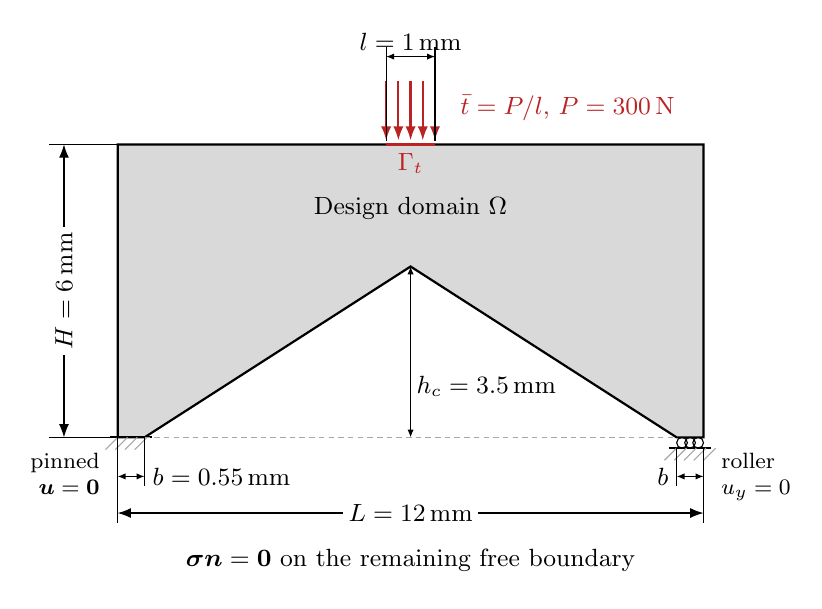
\begin{tikzpicture}[x=0.62cm,y=0.62cm,>=Latex,font=\small,
load/.style={loadred,thick,-{Latex[length=1.8mm,width=1.3mm]}},
dim/.style={thin,<->,>={Latex[length=1mm,width=0.8mm]}}]
\def\L{12}\def\H{6}\def\b{0.55}\def\hc{3.5}\def\l{1}
% Design domain: rectangle minus the triangular notch (b,0)-(L/2,h_c)-(L-b,0)
\draw[thick,fill=black!15]
  (0,0) -- (\b,0) -- (\L/2,\hc) -- (\L-\b,0) -- (\L,0) -- (\L,\H) -- (0,\H) -- cycle;
\node[align=center] at (\L/2,\H-1.3) {Design domain $\Omega$};
% Left support [0,b]: pinned, u = 0
\draw[thick] (-0.15,0) -- (\b+0.15,0);
\foreach \x in {0,0.2,0.4,0.6} \draw[gray!70] (\x,0) -- (\x-0.25,-0.25);
% Right support [L-b,L]: roller, u_y = 0
\foreach \x in {11.56,11.725,11.89} \draw[thin] (\x,-0.11) circle[radius=0.11];
\draw[thick] (\L-\b-0.15,-0.22) -- (\L+0.15,-0.22);
\foreach \x in {11.45,11.65,...,12.25} \draw[gray!70] (\x,-0.22) -- (\x-0.25,-0.47);
% Support labels, outside the domain next to each support
\node[anchor=north east,align=right,inner sep=1pt,font=\footnotesize] at (-0.3,-0.25)
  {pinned\\$\boldsymbol u=\boldsymbol 0$};
\node[anchor=north west,align=left,inner sep=1pt,font=\footnotesize] at (\L+0.3,-0.25)
  {roller\\$u_y=0$};
% Loaded segment Gamma_t on the top edge, centred at x = L/2, width l
\draw[loadred,line width=1.4pt] (\L/2-\l/2,\H) -- (\L/2+\l/2,\H);
\foreach \x in {-0.5,-0.25,0,0.25,0.5}
  \draw[load] (\L/2+\x,\H+1.3) -- (\L/2+\x,\H+0.08);
\node[loadred,anchor=north,inner sep=1pt] at (\L/2,\H-0.12) {$\Gamma_t$};
\node[loadred,align=left,anchor=west,inner sep=1pt] at (\L/2+0.95,\H+0.75)
  {$\bar t=P/l$, $P=300\,\mathrm N$};
% Dimension l
\draw[thin] (\L/2-\l/2,\H+0.08) -- (\L/2-\l/2,\H+2.0);
\draw[thin] (\L/2+\l/2,\H+0.08) -- (\L/2+\l/2,\H+2.0);
\draw[dim] (\L/2-\l/2,\H+1.8) -- (\L/2+\l/2,\H+1.8)
  node[midway,above,inner sep=2pt] {$l=1\,\mathrm{mm}$};
% Dimension H
\draw[thin] (-0.15,0) -- (-1.4,0);
\draw[thin] (0,\H) -- (-1.4,\H);
\draw[thin,<->] (-1.1,0) -- (-1.1,\H)
  node[midway,fill=white,rotate=90,inner sep=2pt] {$H=6\,\mathrm{mm}$};
% Dimension h_c, measured from the support line y = 0
\draw[thin,gray!70,dash pattern=on 2pt off 1.5pt] (\b,0) -- (\L-\b,0);
\draw[dim] (\L/2,0) -- (\L/2,\hc)
  node[pos=0.3,right,inner sep=2pt] {$h_c=3.5\,\mathrm{mm}$};
% Dimensions b (both supports)
\draw[thin] (\b,0) -- (\b,-1.0);
\draw[dim] (0,-0.8) -- (\b,-0.8);
\node[anchor=west,inner sep=1pt] at (\b+0.1,-0.8) {$b=0.55\,\mathrm{mm}$};
\draw[thin] (\L-\b,-0.22) -- (\L-\b,-1.0);
\draw[dim] (\L-\b,-0.8) -- (\L,-0.8);
\node[anchor=east,inner sep=1pt] at (\L-\b-0.1,-0.8) {$b$};
% Dimension L
\draw[thin] (0,0) -- (0,-1.75);
\draw[thin] (\L,-0.22) -- (\L,-1.75);
\draw[thin,<->] (0,-1.55) -- (\L,-1.55)
  node[midway,fill=white,inner sep=2pt] {$L=12\,\mathrm{mm}$};
\node[align=center,anchor=north] at (\L/2,-2.1)
  {$\boldsymbol\sigma\boldsymbol n=\boldsymbol 0$ on the remaining free boundary};
\end{tikzpicture}
\end{document}
